\documentclass[preprint,3p,number]{elsarticle}

\usepackage{amsmath}
\usepackage{amssymb}
\usepackage{subcaption}
% \usepackage{hyperref}
\usepackage{graphicx}
\usepackage{tikz}
\usepackage{pgfplots}
\usepackage{booktabs}
\usepackage{siunitx}
\usepackage[noabbrev,capitalize]{cleveref}
\usepackage{lipsum}

% Tikz libraries
\usetikzlibrary{arrows.meta,patterns,calc}

\bibliographystyle{elsarticle-num}

\begin{document}

\title{Air cavity benchmark for natural convection}
\maketitle

\section{Objective}

\begin{itemize}
    \item Establish that the coupled flow-temperature solver reproduces standard
    natural convection behavior in a square cavity.
\end{itemize}

\section{Goal}

\begin{itemize}
    \item Benchmark Nusselt numbers and velocity extrema agree within a stated
    tolerance; mesh convergence and heat balance are demonstrated.
\end{itemize}

\section{Problem configuration}

\begin{figure}[htbp]
    \centering
    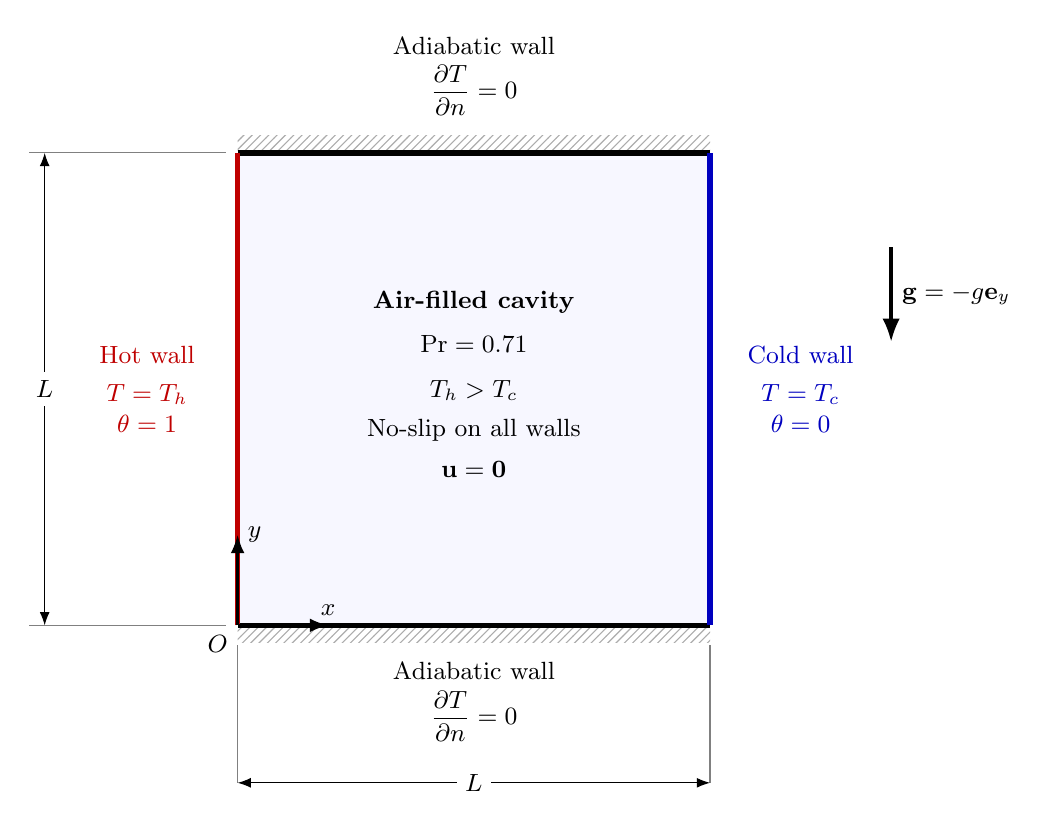
\begin{tikzpicture}[
            >=Latex,
            font=\small,
            wall/.style={line width=2pt},
            dimension/.style={<->,thin},
            extension/.style={thin,gray}
        ]

        % Geometry: square cavity
        \def\L{6}

        % Fluid domain
        \fill[blue!3] (0,0) rectangle (\L,\L);

        % Insulation hatching outside the horizontal walls
        \fill[pattern=north east lines,pattern color=gray!65]
            (0,-0.22) rectangle (\L,0);
        \fill[pattern=north east lines,pattern color=gray!65]
            (0,\L) rectangle (\L,{\L+0.22});

        % Boundary walls
        \draw[wall] (0,0) -- (\L,0);
        \draw[wall] (0,\L) -- (\L,\L);
        \draw[wall,red!75!black] (0,0) -- (0,\L);
        \draw[wall,blue!75!black] (\L,0) -- (\L,\L);

        % Thermal boundary conditions
        \node[align=center,text=red!75!black]
            at (-1.15,3)
            {Hot wall\\[3pt]$T=T_h$\\$\theta=1$};

        \node[align=center,text=blue!75!black]
            at (7.15,3)
            {Cold wall\\[3pt]$T=T_c$\\$\theta=0$};

        \node[above,align=center] at (3,6.35)
            {Adiabatic wall\\[3pt]
            $\displaystyle \frac{\partial T}{\partial n}=0$};

        \node[below,align=center] at (3,-0.35)
            {Adiabatic wall\\[3pt]
            $\displaystyle \frac{\partial T}{\partial n}=0$};

        % Fluid and velocity boundary conditions
        \node[align=center] at (3,3.55)
            {\textbf{Air-filled cavity}\\[5pt]
            $\mathrm{Pr}=0.71$\\[5pt]
            $T_h>T_c$};

        \node[align=center] at (3,2.25)
            {No-slip on all walls\\[4pt]
            $\mathbf{u}=\mathbf{0}$};

        % Gravity
        \draw[->,very thick] (8.3,4.8) -- (8.3,3.6)
            node[midway,right] {$\mathbf{g}=-g\mathbf{e}_y$};

        % Coordinate axes inside the cavity
        \coordinate (O) at (0,0);
        \draw[->,thick] (O) -- (1.15,0)
            node[above] {$x$};
        \draw[->,thick] (O) -- (0,1.15)
            node[right] {$y$};
        \node[below left] at (O) {$O$};

        % Horizontal dimension
        \draw[extension] (0,-0.25) -- (0,-2);
        \draw[extension] (\L,-0.25) -- (\L,-2);
        \draw[dimension] (0,-2) -- (\L,-2)
            node[midway,fill=white,inner sep=3pt] {$L$};

        % Vertical dimension
        \draw[extension] (-0.15,0) -- (-2.65,0);
        \draw[extension] (-0.15,\L) -- (-2.65,\L);
        \draw[dimension] (-2.45,0) -- (-2.45,\L)
            node[midway,fill=white,inner sep=3pt] {$L$};

    \end{tikzpicture}
    \caption{Physical configuration and boundary conditions
    for the differentially heated air-filled square cavity.
    All walls are stationary and impermeable.}
    \label{fig:step0_setup}
\end{figure}

\section{Findings}

\begin{table}[htbp]
    \centering
    \caption{Mesh convergence at $Ra = 10^{6}$ and $Pr = 0.71$.
    Percentage changes are calculated relative to the next finer mesh.}
    \label{tab:mesh_convergence}
    \begin{tabular}{lrrrrrr}
        \toprule
        Mesh &
        $\overline{Nu}_h$ &
        $\delta_{Nu}$ (\%) &
        $U_{\max}$ &
        $\delta_U$ (\%) &
        $V_{\max}$ &
        $\delta_V$ (\%) \\
        \midrule
        $32 \times 32$   & 8.203 & 5.56 & 65.085 & 0.28 & 217.92 & 0.9 \\
        $64 \times 64$   & 8.686 & 1.32 & 64.903 & 0.08 & 219.91 & 0.13 \\
        $128 \times 128$ & 8.802 & 0.22 & 64.848 & 0.02 & 220.20 & 0.0  \\
        $256 \times 256$ & 8.822 & --- & 64.836 & ---  & 220.20 & --- \\
        \bottomrule
    \end{tabular}
\end{table}

\begin{table}[htbp]
    \centering
    \caption{Comparison with the de Vahl Davis (1983)
    benchmark at $Pr=0.71$ \cite{davis1983}. The reference Nusselt number
    is averaged along the hot wall.}
    \label{tab:benchmark_validation}
    \begin{tabular}{llrrr}
        \toprule
        $Ra$ & Quantity & Present & Reference & Error (\%) \\
        \midrule
        $10^3$ & $\overline{Nu}_h$ & 1.118 & 1.117 & 0.09 \\
               & $U_{\max}$       & 3.649 & 3.649 & 0.00 \\
               & $V_{\max}$       & 3.697 & 3.697 & 0.00 \\
        \midrule
        $10^4$ & $\overline{Nu}_h$ & 2.245 & 2.238 & 0.31\\
               & $U_{\max}$       & 16.183 & 16.178 & 0.03 \\
               & $V_{\max}$       & 19.625 & 19.617 & 0.04 \\
        \midrule
        $10^5$ & $\overline{Nu}_h$ & 4.520 & 4.509 & 0.24 \\
               & $U_{\max}$       & 34.74 & 34.73 & 0.03 \\
               & $V_{\max}$       & 68.63 & 68.59 & 0.06 \\
        \midrule
        $10^6$ & $\overline{Nu}_h$ & 8.802 & 8.817 & 0.17 \\
               & $U_{\max}$       & 64.85 & 64.63 & 0.34 \\
               & $V_{\max}$       & 220.20 & 219.36 & 0.38 \\
        \bottomrule
    \end{tabular}
\end{table}

\begin{table}[htbp]
    \centering
    \caption{Steady-state heat balance at $Pr=0.71$.
    Heat input and output are reported as positive magnitudes.}
    \label{tab:heat_balance}
    \begin{tabular}{lrrr}
        \toprule
        $Ra$ & $Q_{\mathrm{in}}$ & $Q_{\mathrm{out}}$
             & $\varepsilon_Q$ (\%) \\
        \midrule
        $10^3$ & 0.00013 & 0.00013 & 0.0 \\
        $10^4$ & 0.00062 & 0.00062 & 0.0 \\
        $10^5$ & 0.00252 & 0.00252 & 0.0 \\
        $10^6$ & 0.01070 & 0.01069 & 0.09 \\
        \bottomrule
    \end{tabular}
\end{table}

\begin{figure}[p]
    \centering

    \begin{subfigure}{0.78\textwidth}
        \centering
        \includegraphics[width=\linewidth]{../result/step0_streamfunction_isotherms_1e+03.png}
        \caption{$Ra=10^3$}
    \end{subfigure}

    \medskip
    \begin{subfigure}{0.78\textwidth}
        \centering
        \includegraphics[width=\linewidth]{../result/step0_streamfunction_isotherms_1e+04.png}
        \caption{$Ra=10^4$}
    \end{subfigure}

    \medskip
    \begin{subfigure}{0.78\textwidth}
        \centering
        \includegraphics[width=\linewidth]{../result/step0_streamfunction_isotherms_1e+05.png}
        \caption{$Ra=10^5$}
    \end{subfigure}

    \medskip
    \begin{subfigure}{0.78\textwidth}
        \centering
        \includegraphics[width=\linewidth]{../result/step0_streamfunction_isotherms_1e+06.png}
        \caption{$Ra=10^6$}
    \end{subfigure}

    \caption{Streamlines (left) and isotherms (right) for
    natural convection in a differentially heated square
    cavity at $Pr=0.71$.}
    \label{fig:streamlines_isotherms}
\end{figure}

\begin{figure}
    \centering
    \includegraphics[width=0.9\textwidth]{../result/step0_velocity_profiles.png}
    \caption{Velocity profiles at $x=0.5$ (left) and $y=0.5$ (right) for different Rayleigh numbers.}
    \label{fig:velocity_profiles}
\end{figure}

\begin{figure}
    \centering
    \includegraphics[width=0.5\textwidth]{../result/local_nusselt_hot_wall.png}
    \caption{Local Nusselt number along the hot wall for different Rayleigh numbers.}
    \label{fig:local_nusselt_hot_wall}
\end{figure}

The mesh study at $Ra=10^6$ demonstrates convergence of the mean hot-wall
Nusselt number and the centreline velocity extrema
(\cref{tab:mesh_convergence}). Refinement from $128\times128$ to
$256\times256$ changes $\overline{Nu}_h$ by approximately $0.22\%$, $U_{\max}$
by $0.02\%$, and $V_{\max}$ by an amount that rounds to $0.0\%$ at the reported
precision. These changes satisfy the $1\%$ criterion for these quantities and
support the use of the $128\times128$ mesh for the benchmark comparisons.
Further refinement removes the small near-corner irregularity in the local
Nusselt profile at $Ra=10^6$, highlighting the greater mesh sensitivity of local
wall gradients.

Over $10^3\leq Ra\leq10^6$ at $Pr=0.71$, the maximum reported deviations from
the de Vahl Davis benchmark are $0.31\%$ for $\overline{Nu}_h$, $0.34\%$ for
$U_{\max}$, and $0.38\%$ for $V_{\max}$ (\cref{tab:benchmark_validation}).
The heat imbalance remains below $0.1\%$ in all cases
(\cref{tab:heat_balance}); entries reported as $0.0\%$ indicate agreement
to the displayed precision rather than necessarily exact equality.

The flow and temperature fields, together with the centreline velocity profiles,
illustrate the increasingly important role of convection as $Ra$ increases
(\cref{fig:streamlines_isotherms,fig:velocity_profiles}). The local Nusselt
profiles exhibit stronger heat transfer near the lower portion of the hot wall,
with a pronounced maximum slightly above the bottom corner at higher $Ra$,
followed by a decrease towards the top
(\cref{fig:local_nusselt_hot_wall}). Taken together, these results
validate the solver for the present air-filled cavity benchmark and provide a
basis for extending the model to cavities containing internal heated cylinders.
The modified geometries will require their own mesh convergence checks.

\bibliography{refs}

\end{document}